%**************************************************************************************
% License:
% CC BY-NC-SA 4.0 (http://creativecommons.org/licenses/by-nc-sa/4.0/)
%**************************************************************************************

\documentclass[notes]{beamer}

\mode<presentation> {

\usetheme{Madrid}

% Burnt orange
\definecolor{burntorange}{rgb}{0.8, 0.33, 0.0}
\colorlet{beamer@blendedblue}{burntorange}
% Pale yellow
\definecolor{paleyellow}{rgb}{1.0, 1.0, 0.953}
\setbeamercolor{background canvas}{bg=paleyellow}
% Secondary and tertiary palett
\setbeamercolor*{palette secondary}{use=structure,fg=white,bg=burntorange!80!black}
\setbeamercolor*{palette tertiary}{use=structure,fg=white,bg=burntorange!60!black}

% To remove the footer line in all slides uncomment this line
%\setbeamertemplate{footline}
% To replace the footer line in all slides with a simple slide count uncomment this line
%\setbeamertemplate{footline}[page number]

% To remove the navigation symbols from the bottom of all slides uncomment this line
%\setbeamertemplate{navigation symbols}{}
}

\usepackage{amsmath}
\usepackage{bm}
\usepackage{breqn}
\usepackage{graphicx} % for figures
\usepackage{subcaption} % for subplots 
\usepackage[labelsep=space,tableposition=top]{caption}
\renewcommand{\figurename}{Fig.} 
\usepackage{cleveref}
\usepackage{caption,subcaption}% http://ctan.org/pkg/{caption,subcaption}
\usepackage{booktabs} % Allows the use of \toprule, \midrule and \bottomrule in tables


% To print 2 slides on a page
%\usepackage{handoutWithNotes}
%\pgfpagesuselayout{2 on 1}[border shrink=2mm]
%----------------------------------------------------------------------------------------
%	TITLE PAGE
%----------------------------------------------------------------------------------------
% The short title appears at the bottom of every slide, the full title is only on the title page
\title[CE394M: Intro to FEM]{CE394M: Introduction to the Finite Element Method} 
\author{Krishna Kumar} % name
\institute[UT Austin] % institution 
{
University of Texas at Austin \\
\medskip
\textit{
  \url{krishnak@utexas.edu}} % Your email address
}
\date{\today} % Date, can be changed to a custom date

\begin{document}

\begin{frame}
\titlepage % title page as the first slide
\end{frame}

\begin{frame}
 % Table of contents slide, comment this block out to remove it
 \frametitle{Overview}
 % Throughout your presentation, if you choose to use \section{} and \subsection{} 
 % commands, these %will automatically be printed on this slide as an overview 
 \tableofcontents
\end{frame}

%----------------------------------------------------------------------------------------
% slides
%----------------------------------------------------------------------------------------
%------------------------------------------------
\section{Numerical analysis of engineering problems}
%------------------------------------------------
\begin{frame}
\frametitle{Numerical analysis of engineering problems}
\mode<beamer>{
	\begin{itemize}
		\item Conceptualize the system
		\begin{itemize}
			\item Geometry
			\item Properties
			\item Processes
		\end{itemize}
		\item Describe it mathematically
		\begin{itemize}
			\item Select the relevant differential equations
		\end{itemize}
		\item Solve the equations (numerically)
		\begin{itemize}
			\item Discretize the system
			\item Settle for approximations (numerical techniques)
		\end{itemize}
		\item Interpret the results
	\end{itemize}	
}
\mode<handout>{
	\vspace{5cm}
}
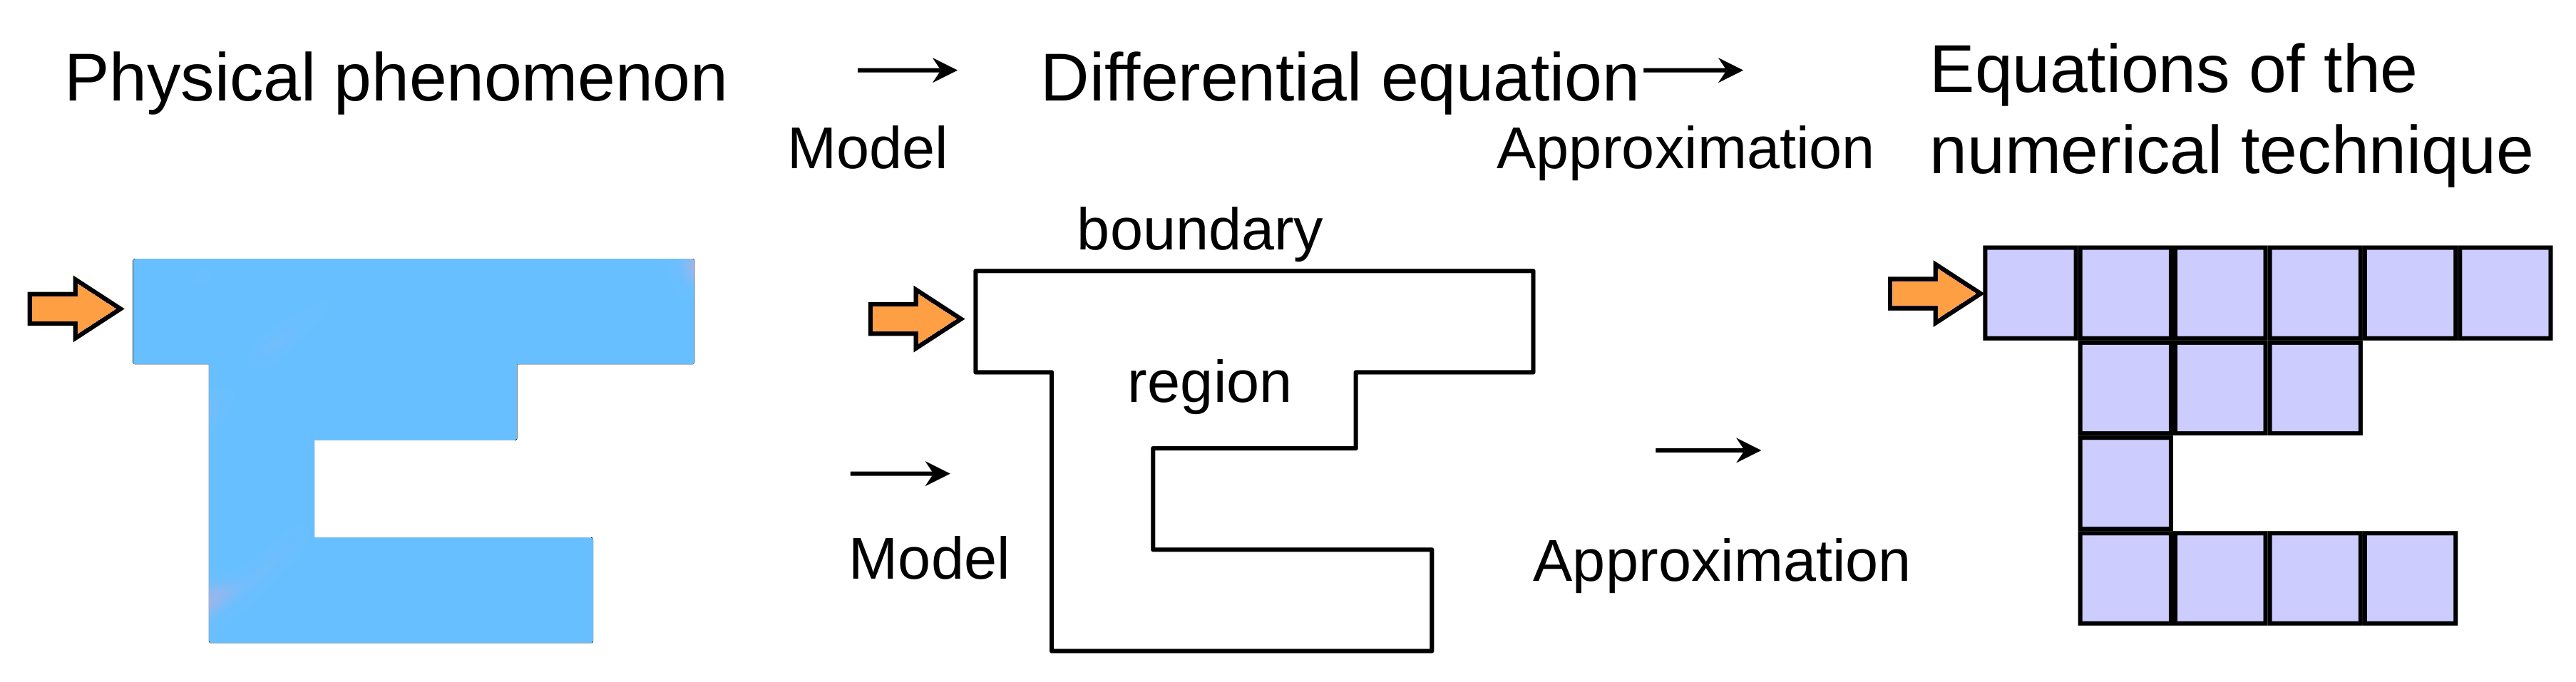
\includegraphics[width=\textwidth]{figs/numerical-pde-workflow.png}
\end{frame}

%------------------------------------------------
\begin{frame}
\frametitle{Boundary value problems}

Differential equations coupled with boundary conditions

\begin{itemize}
\item Steady state (time-independent)
\mode<beamer>{
	\begin{itemize}
		\item Static load-deformation problems: 
		$\partial \sigma / \partial x = 0$ (force + disp. B.C)
		\item Steady seepage state, flow problems: 
		$\partial q / \partial x = 0$ (head + flow B.C)
	\end{itemize}
}
\mode<handout>{
	\vspace{2cm}
}
\item Transient (time-dependent)
\mode<beamer>{
	\begin{itemize}
		\item Consolidation/pore-fluid migration/multiphase flows
		\item Dynamic loading (earthquakes, wave actions)
		\item Contaminant transport processes
	\end{itemize}
}
\mode<handout>{
	\vspace{2cm}
}
\end{itemize}	
\end{frame}


%------------------------------------------------
\begin{frame}
\frametitle{Numerical solutions to differential equations}
\mode<beamer>{
\begin{itemize}
\item Finite differences: Approximate derivatives with expansion into a Taylor series
\item Finite elements
\item Meshless methods
\item Discrete/discontinuous element methods
\item Others...
\end{itemize}
}
\mode<handout>{
\vspace{6cm}
}
\end{frame}


%------------------------------------------------
\begin{frame}
\frametitle{Finite Difference Method}
\mode<beamer>{
	\begin{figure}
		\centering
		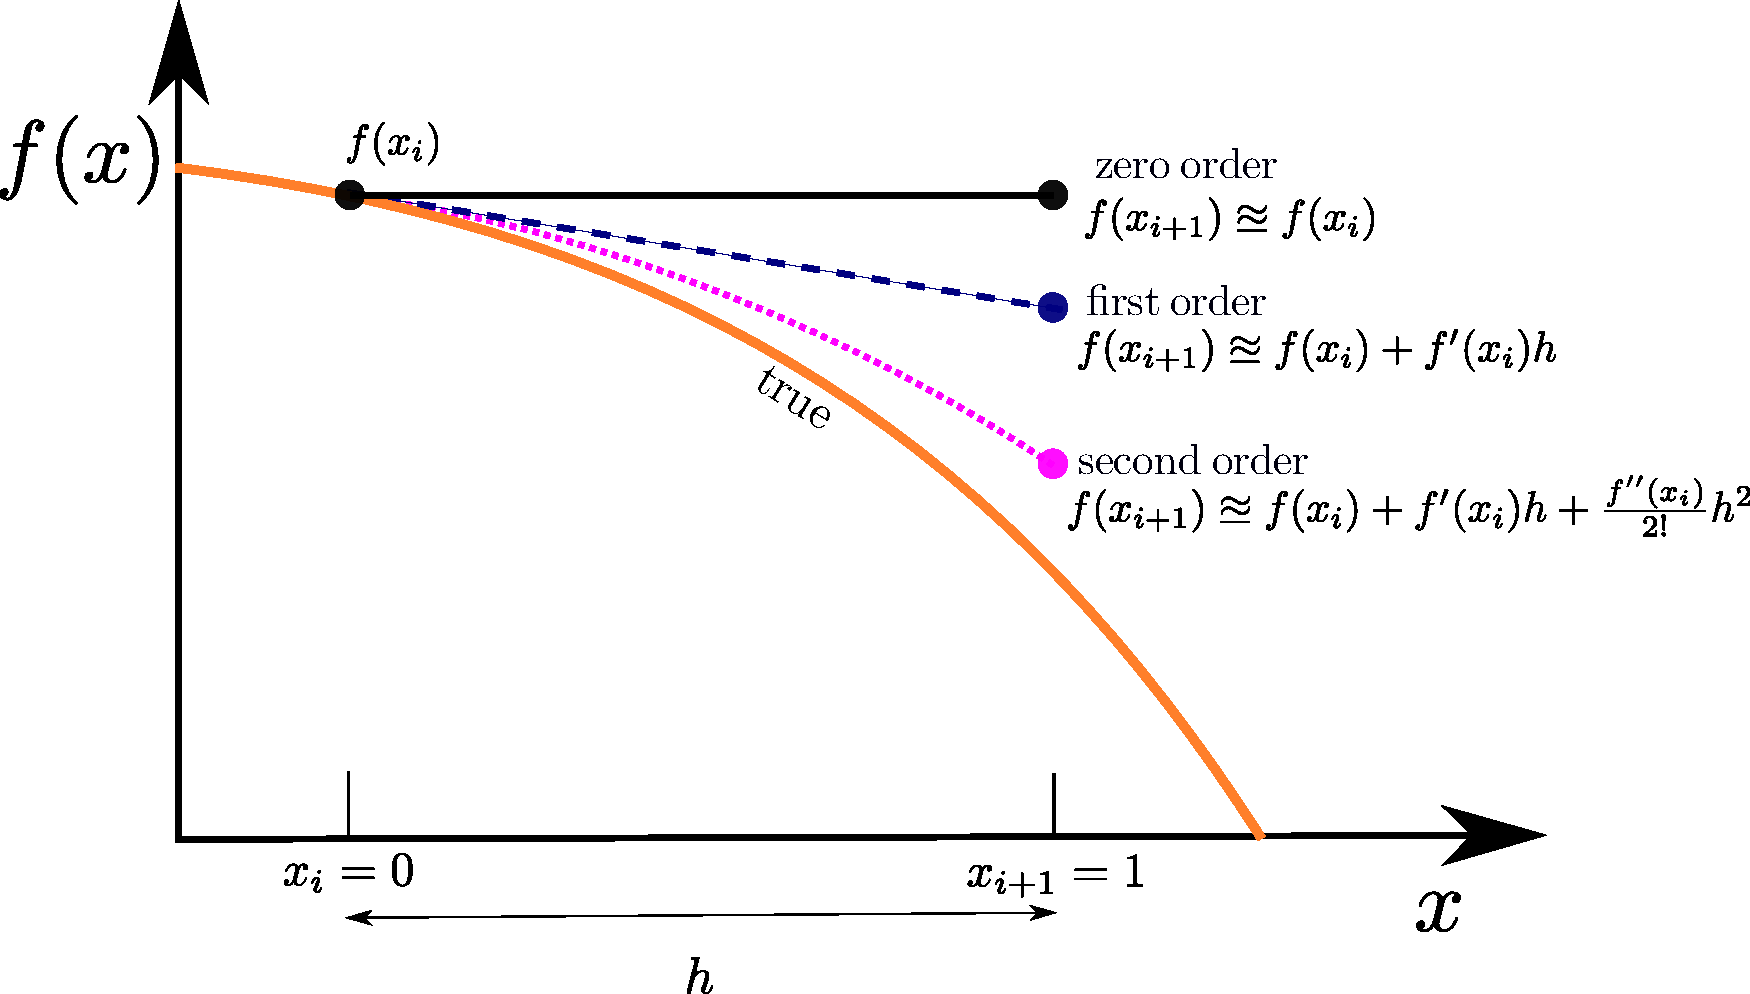
\includegraphics[width=0.8\textwidth]{figs/finite-difference.pdf}
	\end{figure}%
	Expanding Taylor series about the base point of $x=a$:
	\begin{equation*}
		f(x) = \sum_{m=0}^\infty \frac{f^{(m)}(a)}{m!}(x-a)^m = f(a) + f^\prime(a)(x-a) + \frac{f^{\prime\prime}(a)}{2!}(x-a)^2
	\end{equation*}
	
}
\mode<handout>{
	\vspace{6cm}
}
\end{frame}
\note{Differential equation is a continous problem, a computer can only solve a finite problem, 
a discrete problem. So the goal is to take this continous differential equation, like the 
stresses in the soil during an excavation, and solve it as a finite problem. One way is to 
take derivatives and replace by finite differences. So the derivative, the slope of a 
function, in calculus is the exact slope at a point, while the finite differences uses 
the slope between one point and the next point.}

%------------------------------------------------
\begin{frame}
\frametitle{Finite Difference Methods}
\mode<beamer>{
	\begin{figure}
		\centering
		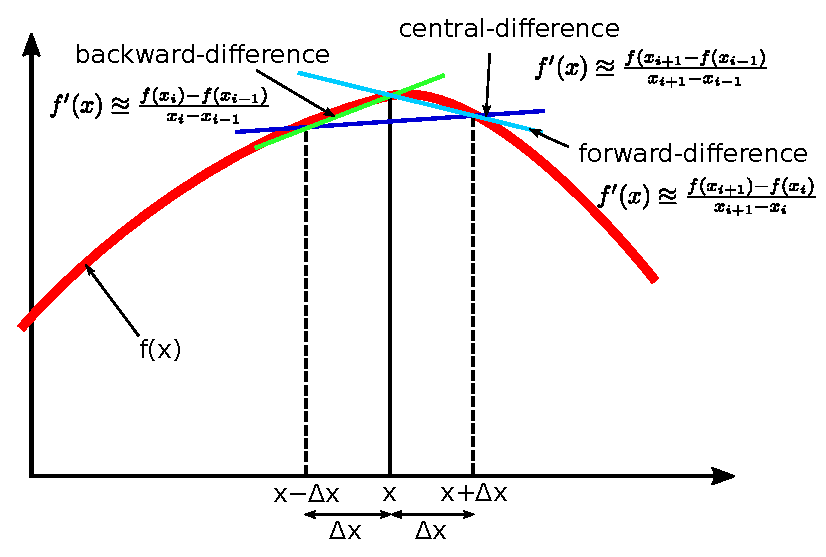
\includegraphics[width=\textwidth]{figs/finite-difference-methods.pdf}
	\end{figure}%
	
}
\mode<handout>{
	\vspace{6cm}
}
\end{frame}

%------------------------------------------------
\begin{frame}
\frametitle{FDM: Groundwater flow}
Darcy's law
\mode<beamer>{
	\begin{equation*}
		q_x = -K \frac{\partial h}{\partial x}, \quad
		q_y = -K \frac{\partial h}{\partial y}
	\end{equation*}%

Continuity equation:
	\begin{equation*}
		 \frac{\partial q_x}{\partial x} + \frac{\partial q_y}{\partial y} = 0
	\end{equation*}%
	
	\begin{equation*}
		\frac{\partial^2 h}{\partial x^2} + \frac{\partial^2 h}{\partial y^2} = 0
	\end{equation*}%

Consider a regularly spaced grid of nodes represented by \textit{i} columns and \textit{j} rows and horizontally and vertically spaced by distances $\delta x$ and $\delta y$. The head at node \textit{i}, \textit{j} is $h_{i,j}$:
	
\begin{align*}
\frac{\partial^2 h}{\partial x^2} & \approxeq \frac{h_{i-1, j} -2 h_{i, j} + h_{i+1, j}}{(\Delta x)^2} \\
\frac{\partial^2 h}{\partial y^2} & \approxeq\frac{h_{i, j-1} -2 h_{i, j} + h_{i, j+1}}{(\Delta y)^2}
\end{align*}%

}
\mode<handout>{
	\vspace{6cm}
}
\end{frame}

\note{
	Adding these two terms according to Laplace’s
	equation and considering \textit{x} and	\textit{y} for a square grid we have:
	\begin{equation*}
		h_{i-1, j} + h_{i+1, j} + h_{i, j-1} + h_{i, j+1} - 4h_{i, j} = 0
	\end{equation*}
	
	\begin{equation*}
	 h_{i, j} = (h_{i-1, j} + h_{i+1, j} + h_{i, j-1} + h_{i, j+1})/4
	\end{equation*}
}

%------------------------------------------------
\begin{frame}
\frametitle{Finite Element Analysis}
\begin{figure}[ht]
	\centering
	\begin{subfigure}[b]{0.4\linewidth}
		\centering
		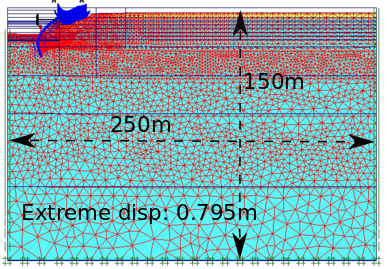
\includegraphics[width=\textwidth]{figs/fea-geotech-mesh.png}
		\caption{FE Mesh}
	\end{subfigure}%
	\begin{subfigure}[b]{0.6\linewidth}
		\centering
		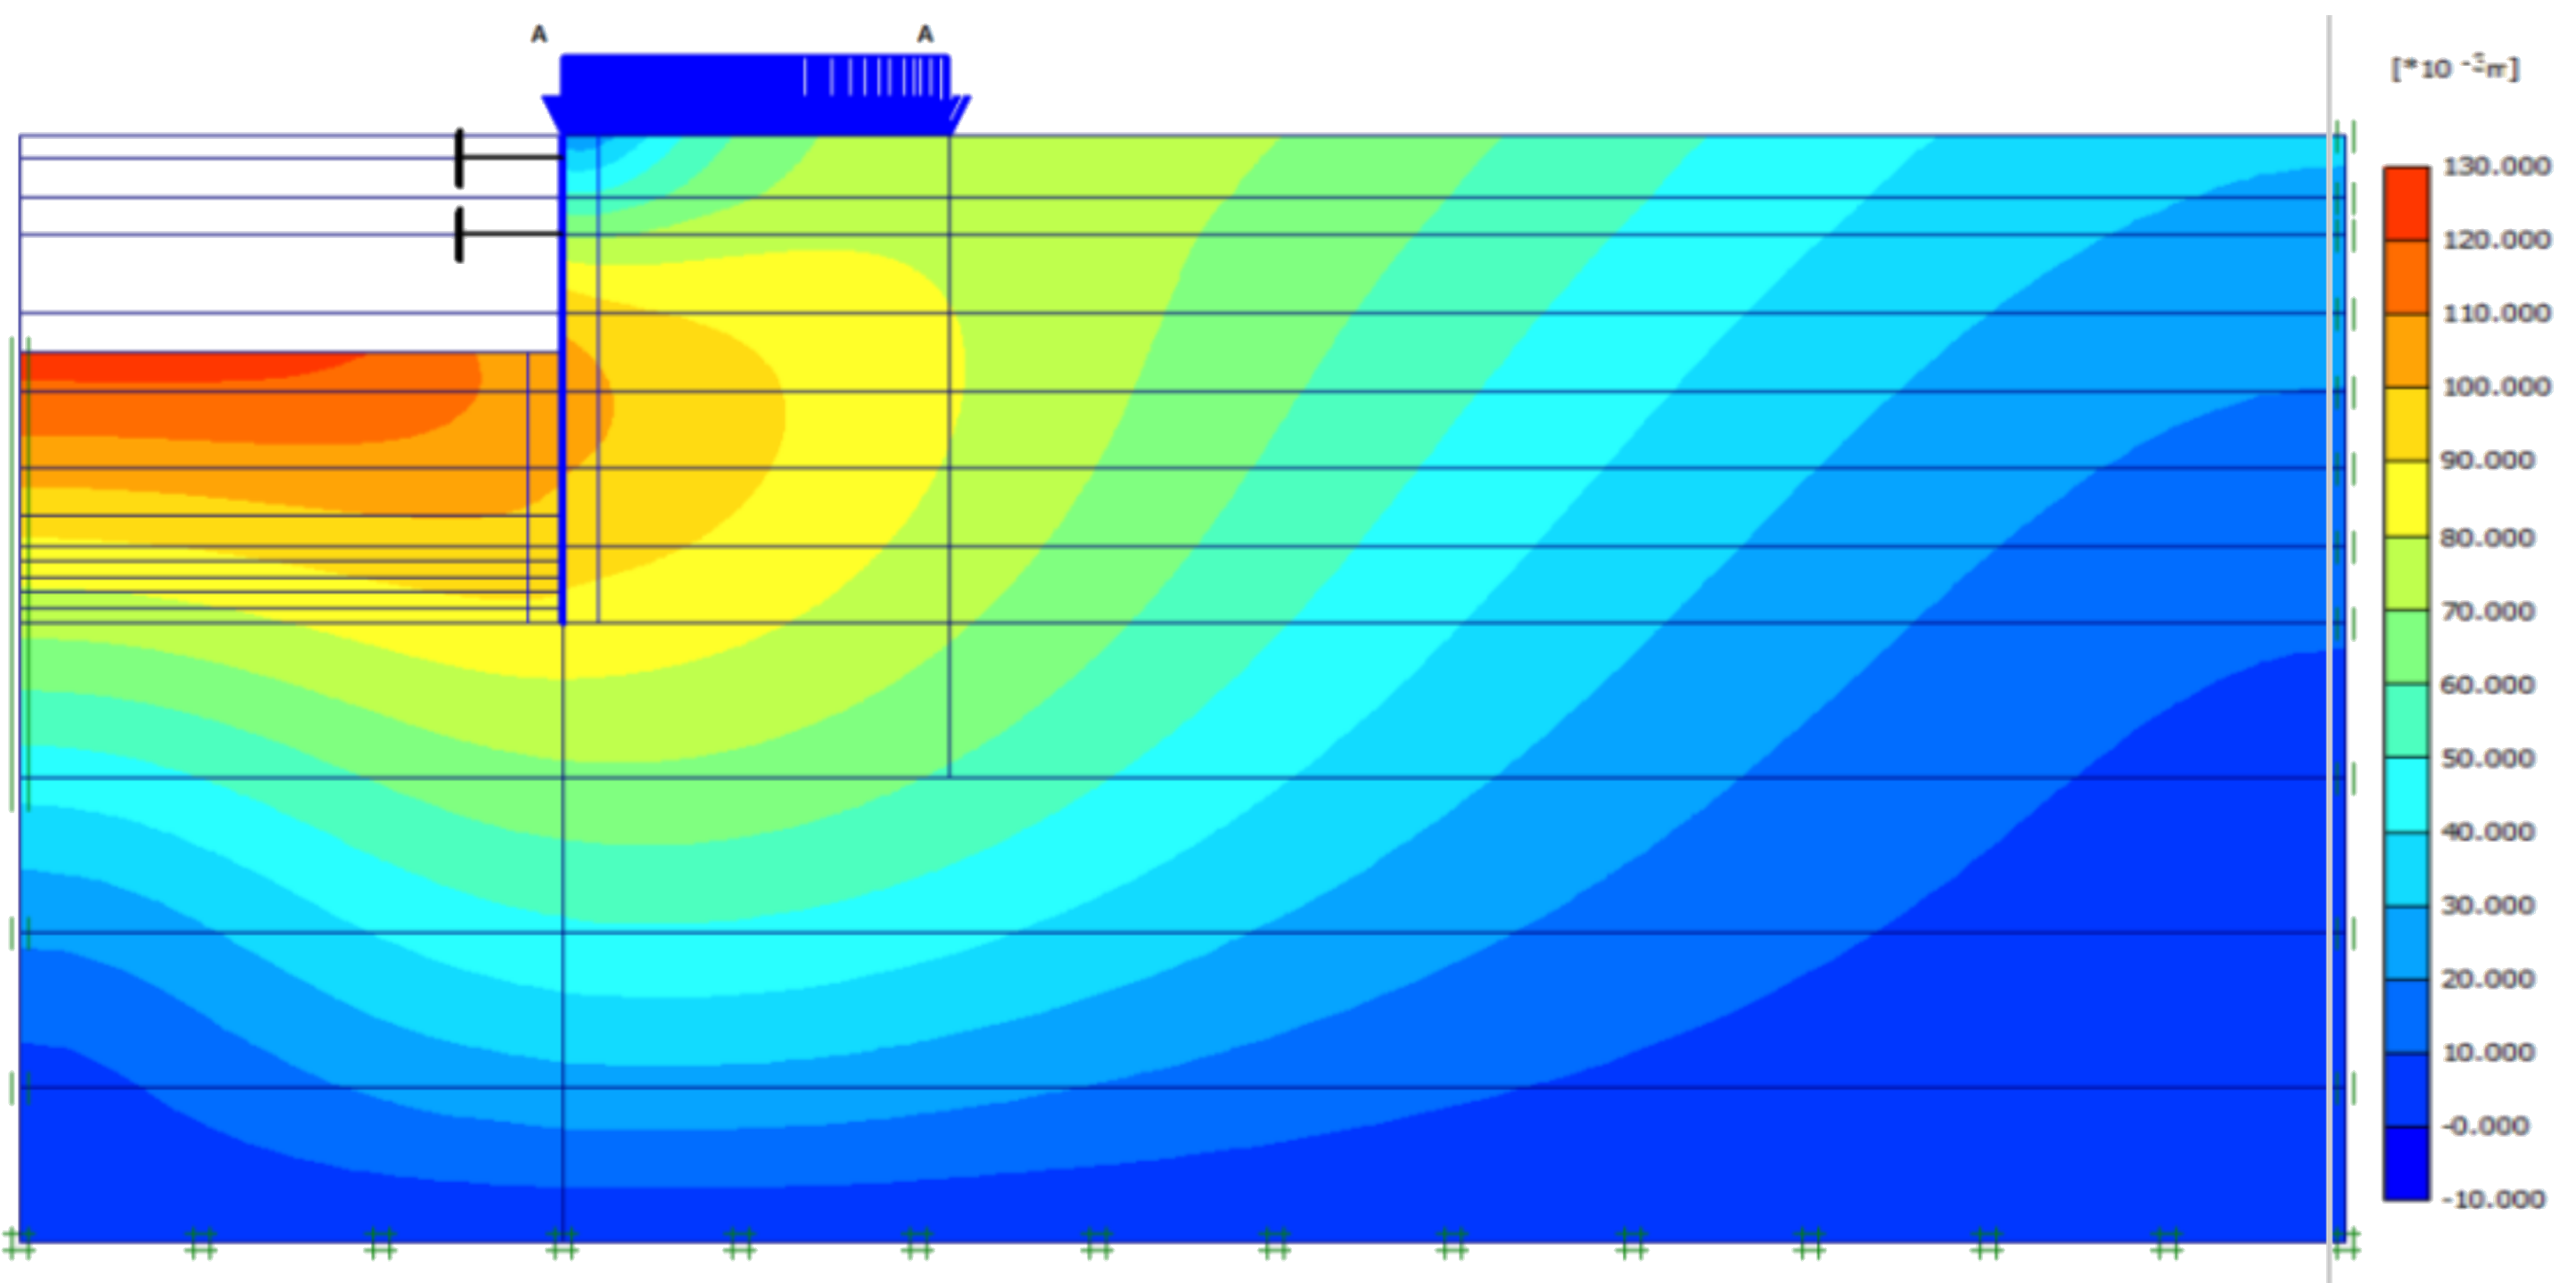
\includegraphics[width=\textwidth]{figs/fea-geotech.png}
		\caption{Displacement profile}
	\end{subfigure}
	\caption*{Singapore Nicoll highway excavation FE analysis}
\end{figure}
\end{frame}

\note{Galerkin is a different one, a different starting point, he took some trial functions, 
	functions that he hoped whose combinations could be close the right answer and the problem 
	then is to find how much of each function goes into the good answer. We are talking about 
	approximations, not exact solutions, geotechnical engineering involves approximations, and 
	is quite OK. 100 years later because of the computers it was possible to work with a hundred 
	thousand functions. Galerkin worked with 2 or 3 trial functions, so he had to make a very 
	close guess of the solution, but if we have a hundred thousand functions they can be just 
	maybe little hat functions, just up and down again simple functions and their combinations, 
	if we have many many can give us close to the correct answer.}

\note{ The whole idea of the FEM is 
	a combination of the Galerkin idea of test functions with the idea of simple functions, where 
	the physics is imple and the equations stay simple, but many many functions and that's what a 
	computer is happy with. So instead of a differential equation, we have a big system to solve.\\
	
	Our unknowns are how much of each hat function goes into the final solution, it's the 
	coefficients we want, the number that multiplies each of the hat functions, when we add 
	them together that we get a big system of equations for those numbers to multiply the 
	hat functions and the system is very well organized for mathematics, so the question is 
	how close is the approximation let's say if I approximate a function like $e^x$ by a 
	thousand hat functions and take a combination of the thousand hat functions to be close 
	to e$^x$, if I take two-thousand hat functions how much closer do I get?}
%------------------------------------------------
\section{Galerkin methods}
%------------------------------------------------
\begin{frame}
\frametitle{Galerkin:Ritz method}
\mode<beamer>{
	\begin{enumerate}
		\item Define the functional $u$ for which you wish to find stationary points.
		\item Choose a combination of linearly independent functions that will be used to 
		approximate the solution. These will be called `basis functions'. The amplitudes of 
		these functions will be the unknowns that you will determine. The basis functions 
		must satisfy the Dirichlet (`fixed') boundary conditions.
		\item Insert the approximate solution into the functional that is now denoted by $u_h$.
		\item Take the directional derivative of $u_h$ with respect to the unknown amplitudes of the
		basis functions.
		\item Determine the amplitudes of the basis functions which yield a stationary point of $u_h$.
	\end{enumerate}
}
\mode<handout>{
	\vspace{5cm}
}
\end{frame}

\note{Numerical methods for partial differential equations are tools for finding approximate
	solutions and are normally used with the aid of a computer. A number of numerical methods 
	are closely linked to a variational form of the differential equation. A group of such methods 
	are known as Galerkin methods. The Ritz method is an example of a Galerkin method, and the 
	finite element method is another. If a numerical method is properly formulated (and the equation 
	is stable), the more effort (read computer time) that is expended, the closer one gets to the 
	exact solution.}

%------------------------------------------------
\begin{frame}
\frametitle{Finite Element Approximations}
\mode<beamer>{
FE approximation of	$u$, which is a dependent variable in a PDE. 

\begin{figure}[ht]
	\centering
	\begin{subfigure}[b]{0.5\linewidth}
		\centering
		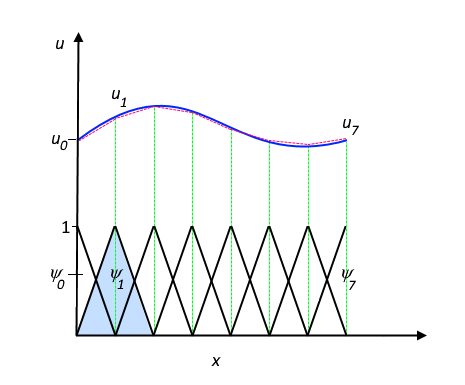
\includegraphics[width=0.8\textwidth]{figs/discretisation2.png}
	\end{subfigure}%
	\begin{subfigure}[b]{0.5\linewidth}
		\centering
		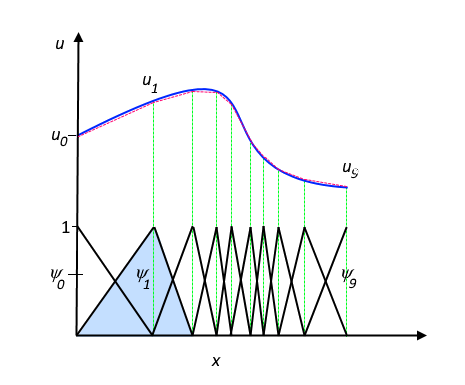
\includegraphics[width=0.8\textwidth]{figs/discretisation1.png}
	\end{subfigure}
	\caption*{FE basis functions}
\end{figure}
The function $u$ can be approximated by a function $u_h$ using linear combinations 
of basis functions according to the following expressions:
\begin{equation*}
u \approx u_h \quad u_h = \sum_{i} u_i \psi_i
\end{equation*}
}
\mode<handout>{
\vspace{5cm}
}
\end{frame}



\note{The reality of partial differential equations is that in most cases it is 
	not possible to find an analytical solution. This is particularly so for 
	equations on complicated geometries (as is common in engineering), nonlinear 
	equations and equations with complicated source terms and boundary conditions.
	
	Instead, an approximation of the equations needs to be constructed, typically 
	based upon different types of discretizations. These discretization methods 
	approximate the PDEs with numerical model equations, which can be solved using 
	numerical methods. The solution to the numerical model equations are, in turn, 
	an approximation of the real solution to the PDEs. The finite element method 
	(FEM) is used to compute such approximations.}

\note{Take, for example, a function $u$ that may be the dependent variable in a PDE 
	(i.e., temperature, electric potential, pressure, etc.) The function $u$ can be 
	approximated by a function uh using linear combinations of basis functions 
	according to the following expressions: 
	
	\begin{equation*}
	u \approx u_h \quad u_h = \sum_{i} u_i \psi_i
	\end{equation*}
	
	Here, $\psi_i$ denotes the basis functions and $u_i$ denotes the coefficients of 
	the functions that approximate u with uh. The figure below illustrates this 
	principle for a 1D problem. $u$ could, for instance, represent the temperature 
	along the length ($x$) of a rod that is nonuniformly heated. Here, the linear basis 
	functions have a value of 1 at their respective nodes and 0 at other nodes. In 
	this case, there are seven elements along the portion of the x-axis, where the 
	function $u$ is defined (i.e., the length of the rod).}

\note{One of the benefits of using the finite element method is that it offers great 
	freedom in the selection of discretization, both in the elements that may be used to 
	discretize space and the basis functions. In the figure above, for example, the elements 
	are uniformly distributed over the x-axis, although this does not have to be the case. 
	Smaller elements in a region where the gradient of u is large could also have been applied.\\
	
	Both of these figures show that the selected linear basis functions include very limited 
	support (nonzero only over a narrow interval) and overlap along the x-axis. Depending on 
	the problem at hand, other functions may be chosen instead of linear functions.\\
	
	\url{https://www.comsol.com/multiphysics/finite-element-method}}

\section{Strong form}

%------------------------------------------------
\begin{frame}
\frametitle{Strong form of the equilibrium equation for a 1-D bar}
\begin{figure}
	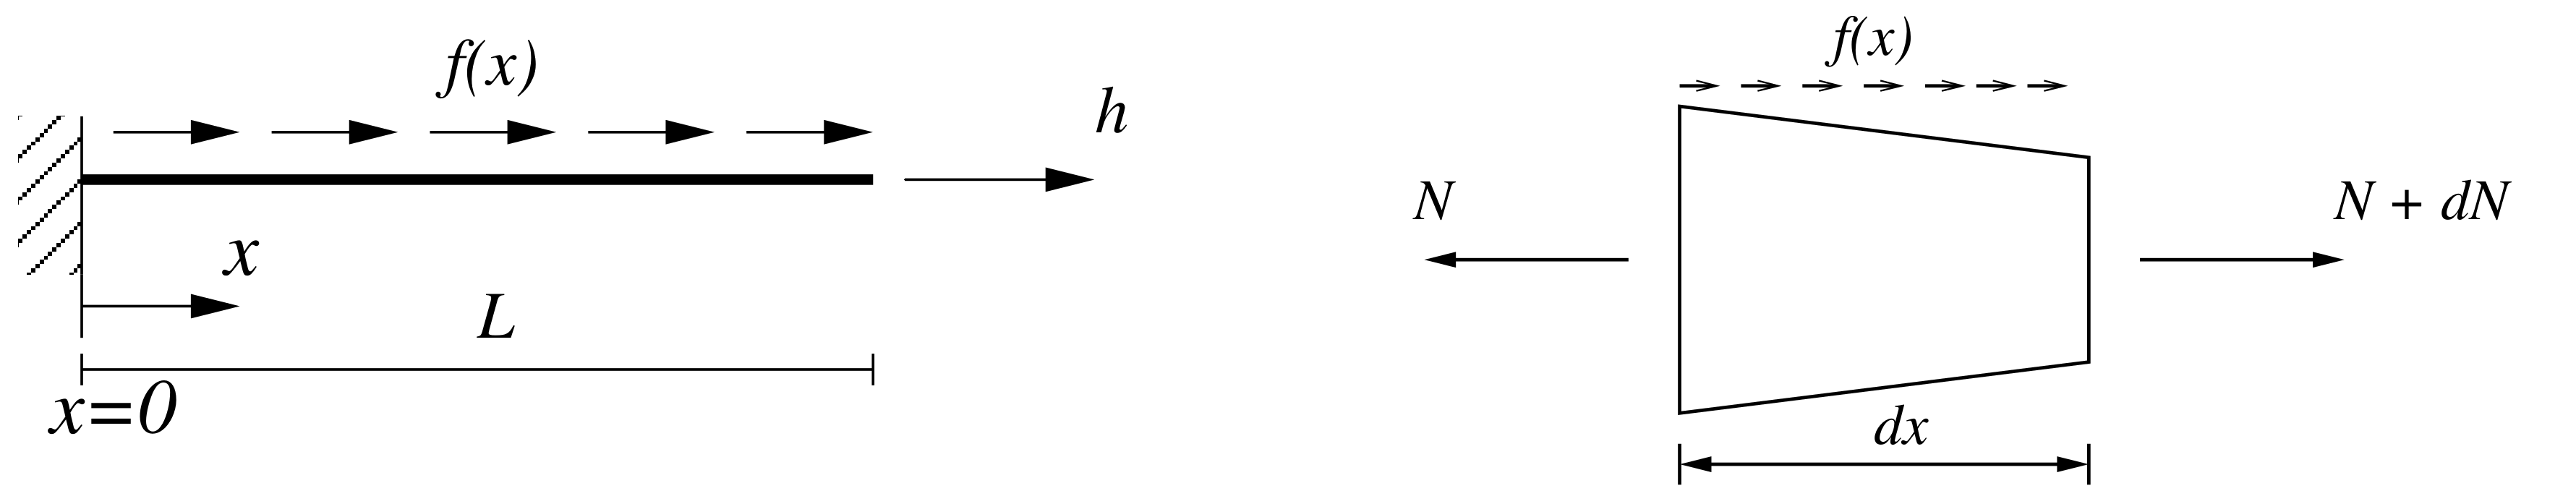
\includegraphics[width=\textwidth]{figs/strong-form-1d-bar.png}
	\caption*{where $f$ is a distributed force and $h$ as a force applied at the end of the bar}
\end{figure}
The equilibrium equation can be derived by considering an infinitesimal bar: 
\mode<beamer>{
	\begin{equation*}
		- \frac{dN}{dx} = f
	\end{equation*}
}
\mode<handout>{
	\vspace{2cm}
}
where $N$ is the normal force in the bar and $f$ is the distributed force along the bar.
\end{frame}

%------------------------------------------------
\begin{frame}
\frametitle{Boundary value problem of a 1-D bar}
For linear elasticity
\mode<beamer>{
	\begin{equation*}
		N = A \sigma = E A \frac{du}{dx} = EA\varepsilon
	\end{equation*}
}
\mode<handout>{
	\vspace{1.5cm}
}
where $A(x)$ is the area of the bar, $E(x)$ is Young’s modulus $u$ is the displacement and $\varepsilon =
du/dx$ is the strain.
\mode<beamer>{
	\begin{equation*}
	- \frac{d}{dx}\left(EA \frac{du}{dx}\right) = f
	\end{equation*}
}
\mode<handout>{
	\vspace{1.5cm}
}
which is a second-order differential equation. BCs:
\mode<beamer>{
	\begin{enumerate}
	\item $u = 0$ at $x = 0$ (displacement or `Dirichlet' boundary condition),
	\item $EA\varepsilon = h$ at $x = L$ (force or `Neumann' boundary condition).
	\end{enumerate}
We now have a well-defined boundary value problem that can be solved.
}
\mode<handout>{
	\vspace{1cm}
}

\end{frame}
\note{
	To formulate a boundary value problem, we need to assume a constitutive model which
	defines the relationship between stress and deformation, and we need to supply boundary
	conditions.

	\textbf{Dirichlet (or first-type) boundary condition} is a type of boundary condition, 
	when imposed on an ordinary or a partial differential equation, it specifies the values 
	that a \textbf{solution needs to take on along the boundary of the domain}.
	
	 \textbf{Neumann (or second-type) boundary condition} is a type of boundary condition, 
	 when imposed on an ordinary or a partial differential equation, the condition specifies 
	 the values in which \textbf{the derivative of a solution is applied within the boundary 
	 	of the domain}. 
}

\section{Weak form}
%------------------------------------------------
\begin{frame}
\frametitle{Weak form of the equilibrium equations of a 1D bar}
The general derivation of the weak form of any equation from the strong form
follows a standard procedure:

\begin{enumerate}
	\item Multiply the strong equation by a weight function $v$ which is equal to zero where
	Dirichlet (displacement) boundary conditions are applied, but is otherwise arbitrary 
	(Another condition is that it must be sufficiently continuous. The degree of continuity 
	required depends on the properties of the equation being considered.)
	\item Use integration by parts to `shift' derivatives to the weight function
	\item Insert the Neumann (force) boundary conditions
\end{enumerate}

We then want to find a solution $u$ to the weak form that holds for all $v$ . The weight
function is also known as the `\textit{test}' function.
\end{frame}

%------------------------------------------------
\begin{frame}
\frametitle{Weak form of the equilibrium equations of a 1D bar}
Multiplying equilibrium equation by an arbitrary weight function v and
integrating along the bar:
\begin{equation*}
-\int_0^L v \frac{dN}{dx}\, \mathrm{d}x. = \int_0^L v f\, \mathrm{d}x.
\end{equation*}
we require that $v(0) = 0$ because of the displacement boundary condition at $x = 0$.
\begin{equation*}
\int_0^L \frac{dv}{dx} N\, \mathrm{d}x. = \int_0^L v f\, \mathrm{d}x + v N |_{x=0}^{x=L}.
\end{equation*}
Since $v(0) = 0$, inserting the constitutive relationship and taking into account the force
boundary condition at $x = L$.
\begin{equation*}
\int_0^L \frac{dv}{dx} EA \frac{du}{dx}\, \mathrm{d}x. = \int_0^L v f\, \mathrm{d}x + v(L)h.
\end{equation*}
The task is to find $u$ with $u(0) = 0$ such that this equation is satisfied for all $v$.
\end{frame}

% Strong vs Weak form
\note{Strong form is the conventional PDE. The strong form imposes continuity and differentiability 
	requirements on the potential solutions to the equation. Weak form is an alternate representation of 
	the differential equation. The weak form relaxes these 
	requirements on solutions to a certain extent. This means that a larger set of 
	functions are solutions of the weak form. By construction all solutions of the strong 
	form satisfy the weak form but not vice-versa. \\

	Weak formulations are often referred to as `variational formulations'. In fact, the weak form 
	is more general than the strong form. 
	The weak form of an equation does not generally make an equation easier to solve 
	analytically (it may make it harder), but is usually a more suitable form for 
	mathematical analysis (allowing us to say things about the properties of the equation 
	without knowing the solution) and for numerical solution methods.}

\note{Weak form asks that the average value of $EA\frac{du}{dx}$ in the entire domain to be 
	equal to the average value of force $f$. Indeed, it seems ``too weak'' as compared to the original 
	differential equation, which asks that at every point $EA\frac{du}{dx}$ should be $f$. 
}

\note{An important observation
	is that the weak form for the bar contains at most first-order derivatives, whereas the
	strong form for this problem contained second-order derivatives. We have transferred
	one derivative from the displacement field $u$ to weight function $v$ using integration by
	parts. This is a key feature of the weak form and is crucial for finite element methods.
	If the symbol $v$ in the weak form was replaced by the symbol $\delta \varepsilon$, 
	the weak form in the case of the bar resembles the virtual work equation. It is in fact 
	equivalent. However, the process that we have followed is general and does not require 
	any knowledge of virtual work, and can be applied to any differential equation.}

%------------------------------------------------
\section{Finite Element formulation}
%------------------------------------------------
\begin{frame}
\frametitle{FE formulation of a 1-D bar}
\mode<beamer>{
Approximates the PDE by replacing the unknown function (the displacement $u$ 
of the elastic bar) and the weight function ($v$) by approximate fields $u_h$ and $v_h$. Inserting these fields into the weak equilibrium equation for a bar:

	\begin{equation*}
	\int_0^L \frac{dv_h}{dx} EA \frac{du_h}{dx}\, \mathrm{d}x. = \int_0^L v_h f\, \mathrm{d}x + v_h(L)h.
	\end{equation*}
	
We now allow only a limited number of possibilities for $v_h$ and $u_h$. 

Therefore, it is now unlikely that $u_h$ will be equal to the exact solution.
}
\mode<handout>{
	\vspace{6cm}
}
\end{frame}

%------------------------------------------------
\begin{frame}
\frametitle{Basis functions}
	The approximate displacement field $u_h$ is represented by a set of `\textit{basis
	functions}' $N_i(x)$:

\mode<beamer>{
	
	\begin{equation*}
		u_h(x) = \sum_i^n N_i(x) a_i
	\end{equation*}

	$x_i$: discrete number of points (known as nodes)\\ 
    $a_i$: degrees of freedom\\
    $n$: number of nodes
}
\mode<handout>{
	\vspace{4cm}
}
The approximate strain field:
\mode<beamer>{
	\begin{equation*}
		\varepsilon_h = \frac{du_h}{dx} = \sum_i^n \frac{dN_i(x)}{dx} a_i
	\end{equation*}
The task of the FE formulation will be to find the coefficients $a_i$, which will the approximate solution $u_h$ and $\varepsilon_h$.
}
\mode<handout>{
	\vspace{2cm}
}
\end{frame}

%------------------------------------------------
\begin{frame}
\frametitle{FE shape functions}
The simplest finite element basis functions in 1D hat-like continuous, piece-wise linear polynomials.

\begin{figure}
	\centering
	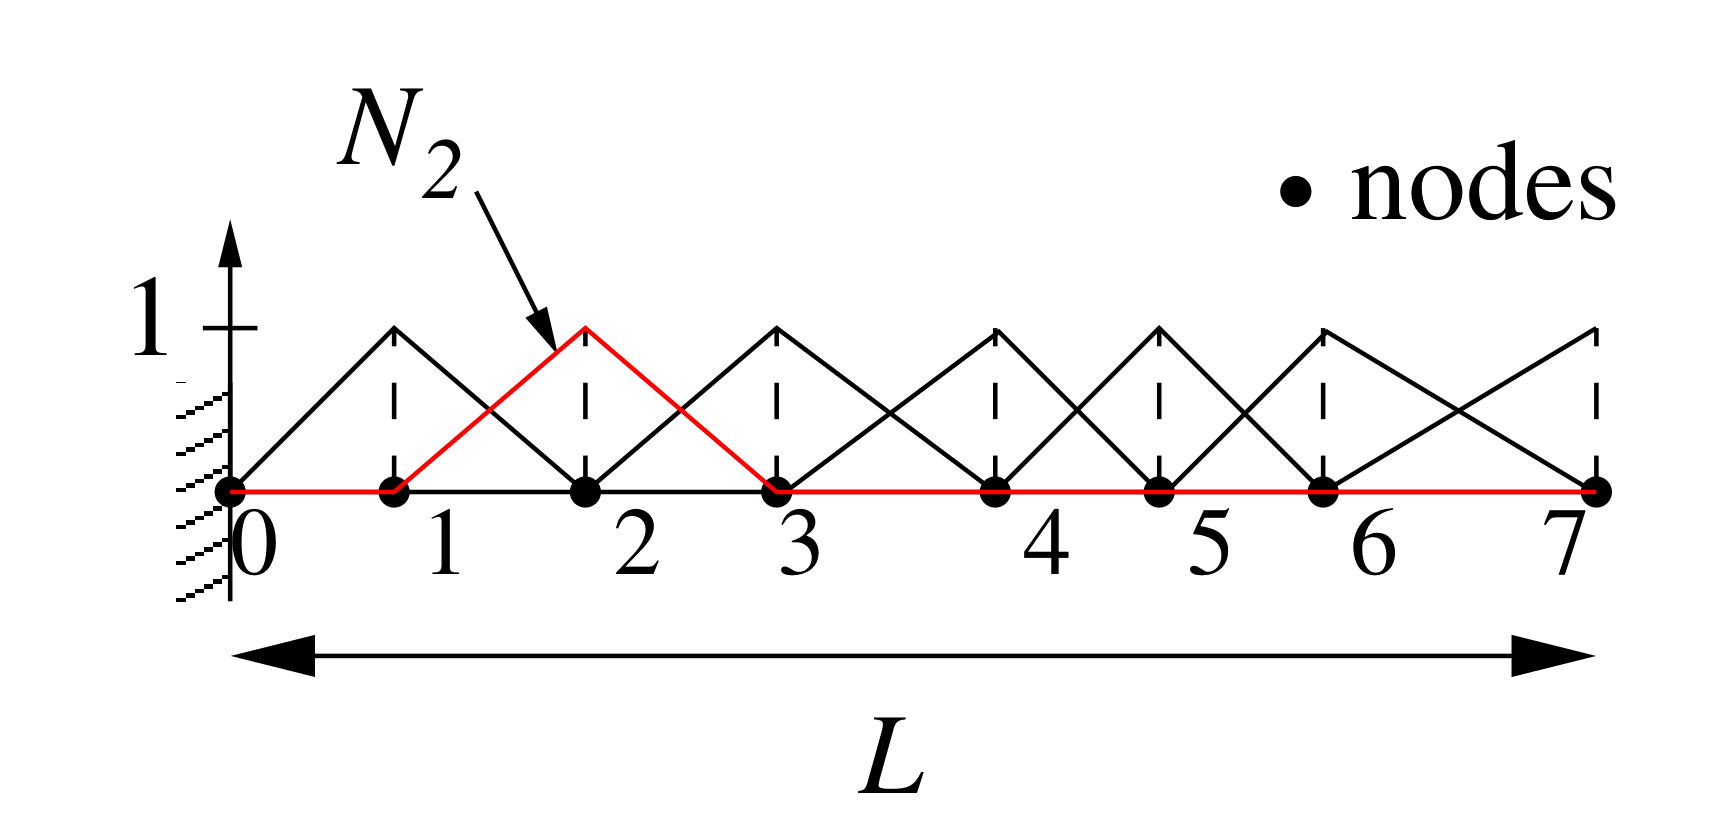
\includegraphics[width=0.5\textwidth]{figs/shape-functions.png}
\end{figure}

\mode<beamer>{
Each node $i$ has its own shape function and its own degree of freedom. A
shape function is equal to one at its own node, and zero at all others.	

\begin{equation*}
N_i(x) = \begin{cases}
\frac{x - x_{i-1}}{x_i - x_{i-1}}\quad x_{i-1} < x \le x_i \,,\\
\frac{x_{i+1} - x}{x_{i+1} - x_i}\quad x_{i} < x < x_{i+1} \,,\\
0 \qquad \quad \mathrm{otherwise.}
\end{cases}
\end{equation*}
}
\mode<handout>{
	\vspace{4cm}
}
\end{frame}


%------------------------------------------------
\begin{frame}
\frametitle{FE shape functions}
For a bar divided into three elements, the displacement and strain fields could have the
form
\mode<beamer>{

\begin{figure}[ht]
	\centering
	\begin{subfigure}[b]{0.5\linewidth}
		\centering
		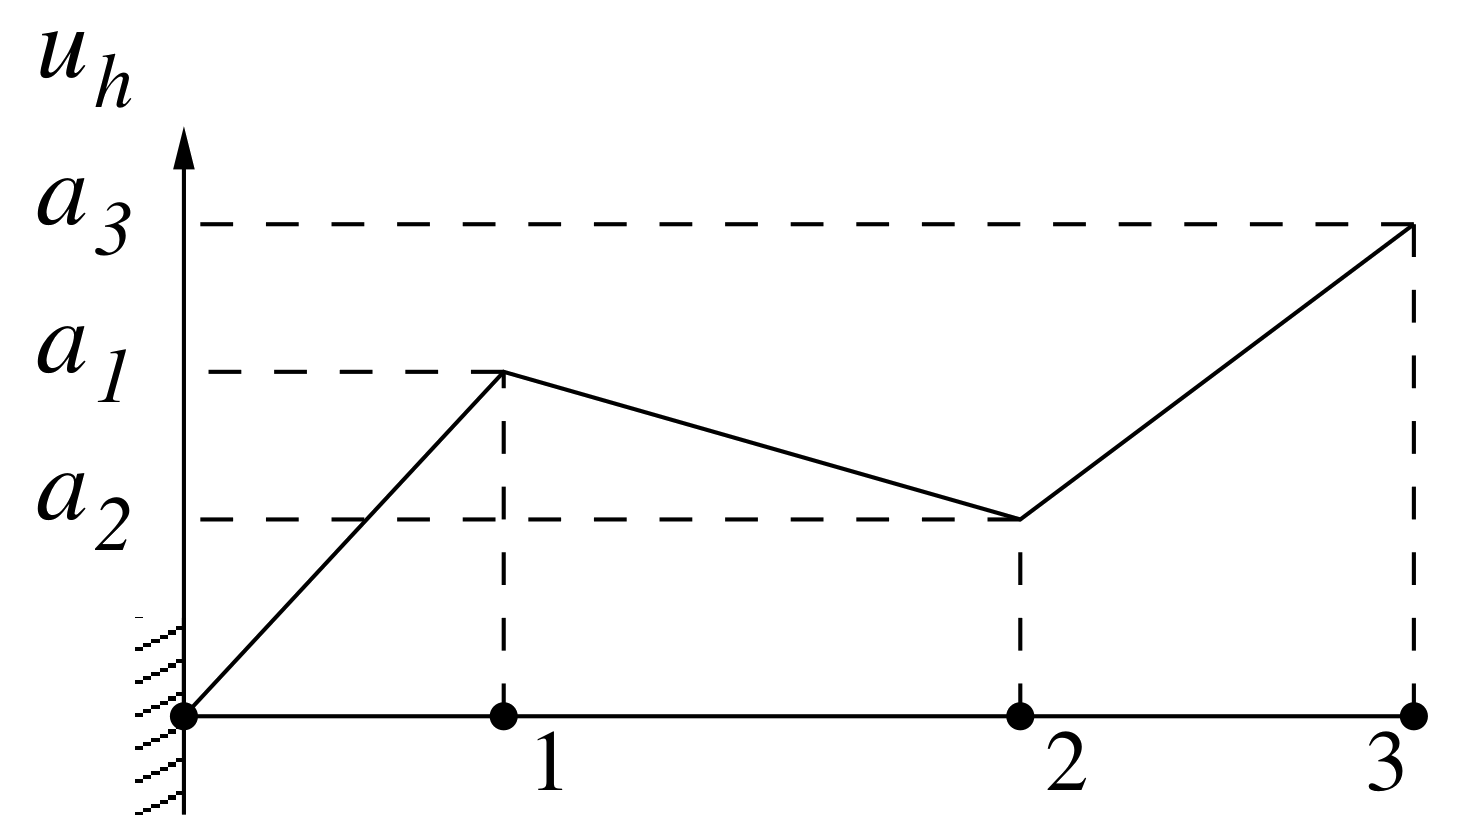
\includegraphics[width=\textwidth]{figs/beam-disp.png}
		\caption{displacement field}
	\end{subfigure}%
	\begin{subfigure}[b]{0.5\linewidth}
		\centering
		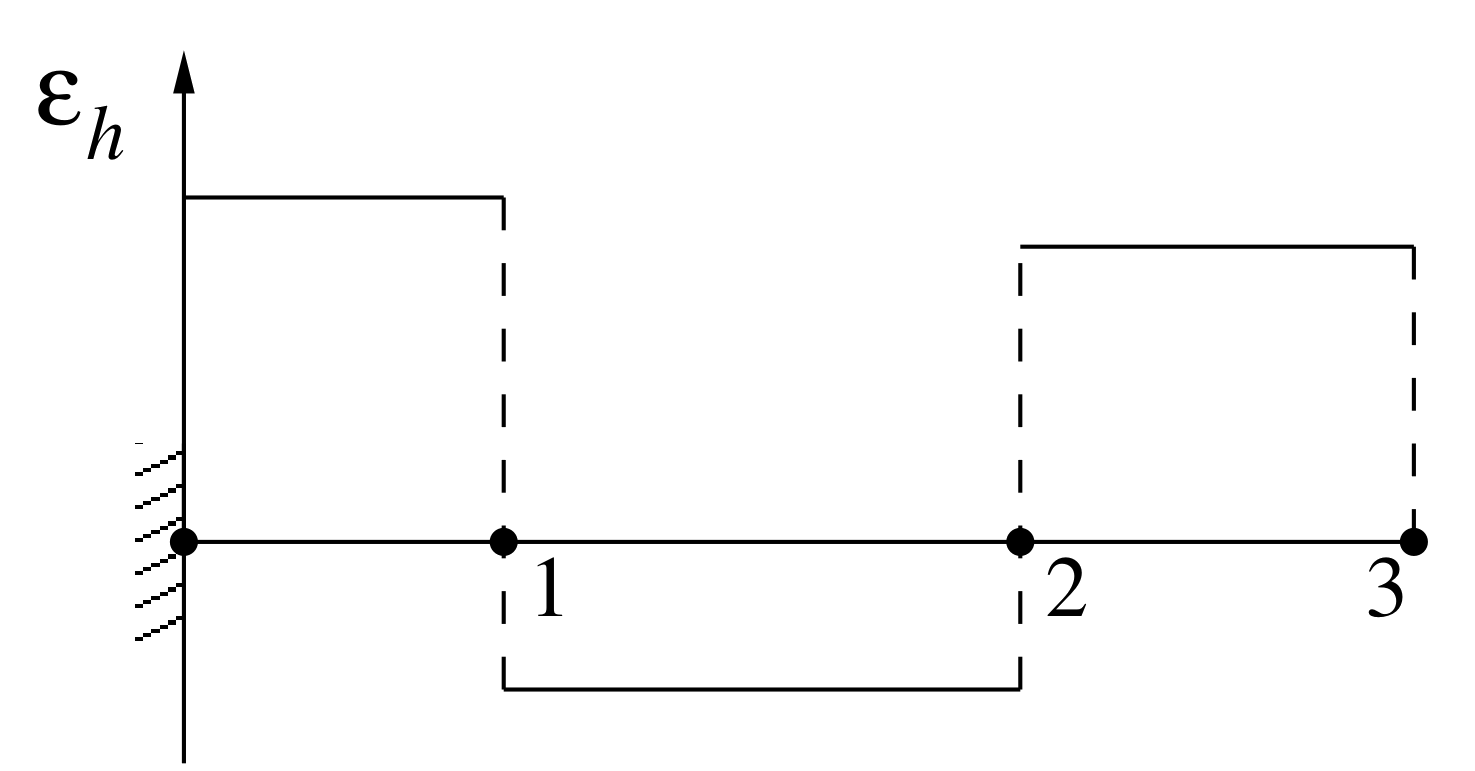
\includegraphics[width=\textwidth]{figs/beam-strains.png}
		\caption{strain field}
	\end{subfigure}
\end{figure}
}
\mode<handout>{
	\vspace{5cm}
}
\end{frame}

%------------------------------------------------
\begin{frame}
\frametitle{FE formulation of a 1-D bar}
Weak form:
\begin{equation*}
\int_0^L EA \frac{dv_h}{dx} \frac{du_h}{dx}\, \mathrm{d}x. = \int_0^L v_h f\, \mathrm{d}x + v_h(L)h.
\end{equation*}
Using basis functions for $u_h$ and $v_h$:
\mode<beamer>{
\begin{multline*}
\int_0^L EA \left(\sum_i^n\frac{dN_i}{dx}\,a_i^*\right) \left(\sum_j^n\frac{dN_j}{dx}\,a_j\right) \, \mathrm{d}x = \int_0^L \left(\sum_i^n N_i a_i^*\right)\,f\,\mathrm{d}x + \\ \left(\sum_i^n N_i(L) a_i^*\right)\,h
\end{multline*}
}
\mode<handout>{
	\vspace{3cm}
}
since $a_i^*$  and $a_j$ are not a function of $x$, we take it out.
\begin{equation*}
	\sum_i^n a_i^* \left(\sum_j^n a_j \int_0^L EA \frac{dN_i}{dx}\frac{dN_j}{dx}\, \mathrm{d}x \right)  = \sum_i^n a_i^* \int_0^L N_i \,f\,\mathrm{d}x + \sum_i^n N_i(L) a_i^*\,h
\end{equation*}
\end{frame}


%------------------------------------------------
\begin{frame}
\frametitle{FE formulation of a 1-D bar}
Since $a_i^*$ is arbitrary for each $i$ we set $a_{k=i}^*=1$ and $a_{k \ne i}^*=0$. Then for each $i$ we have an equation with $n$ unknowns (the values of $a_j$):
\begin{align*}
i = 1: \quad & \sum_j^n {a_j} \int_{0}^{L}EA \frac{dN_1}{dx}\frac{dN_j}{dx} dx = \int_{0}^{L}N_1 f dx + N_i(L)h, \\
i = 2: \quad & \sum_j^n {a_j} \int_{0}^{L}EA \frac{dN_2}{dx}\frac{dN_j}{dx} dx = \int_{0}^{L}N_2 f dx + N_i(L)h, \\
\quad & \vdots \\
i = n: \quad & \sum_j^n {a_j} \int_{0}^{L}EA \frac{dN_n}{dx}\frac{dN_j}{dx} dx = \int_{0}^{L}N_n f dx + N_i(L)h,
\end{align*}
\end{frame}

%------------------------------------------------
\begin{frame}
\frametitle{FE formulation of a 1-D bar}
A system of linear equations is most conveniently expressed as a matrix:

\mode<beamer>{
	\begin{equation*}
		\mathbf{K a} = \mathbf{b}
	\end{equation*}
}
\mode<handout>{
	\vspace{2cm}
}
Stiffness matrix: 
\mode<beamer>{
	\begin{equation*}
	K_{ij} = \int_{0}^{L}EA \frac{dN_i}{dx}\frac{dN_j}{dx} dx
	\end{equation*}
}
\mode<handout>{
	\vspace{2cm}
}
right-hand side vector:
\mode<beamer>{
	\begin{equation*}
		b_i = \int_{0}^{L}N_i f dx + N_i(L)h.
	\end{equation*}
}
\mode<handout>{
	\vspace{2cm}
}
\end{frame}


%------------------------------------------------
\begin{frame}
\frametitle{Finite Element Method: Formulation}
	\begin{align*}
		\left[\mathbf{K}\right]{\textbf{u}} & = {F} \\
		{\textbf{u}} & = \left[\mathbf{K}\right]^{-1} {F}
	\end{align*}
	
\begin{table}[]
	\begin{tabular}{llll}
		\toprule
		& \multicolumn{1}{l}{\textbf{Property {[}K{]}}} & \multicolumn{1}{l}{\textbf{Behavior \{u\}}} & \multicolumn{1}{l}{\textbf{Action \{F\}}} \\
		\midrule
		\textbf{Elastic} & stiffness                                     & displacement                                 & force                                     \\
		\textbf{Thermal} & conductivity                                  & temperature                                  & heat source                               \\
		\textbf{Fluid}   & viscosity                                     & velocity                                     & body force       						 \\
		\bottomrule                        
	\end{tabular}
\end{table}
\end{frame}


%------------------------------------------------
\section{Shape functions}
%------------------------------------------------
\begin{frame}
\frametitle{Linear shape functions}
\begin{figure}
	\centering
	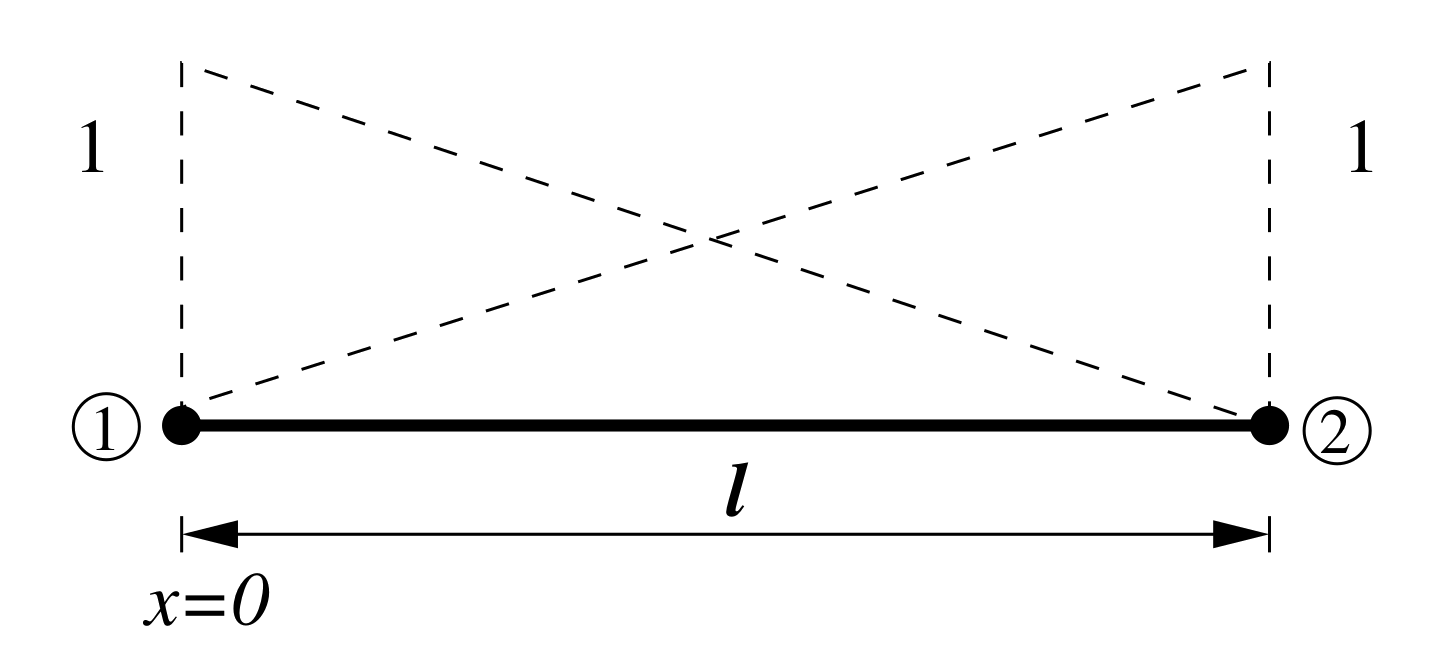
\includegraphics[width=0.6\textwidth]{figs/1d-shape-function.png}
\end{figure}

\mode<beamer>{A polynomial shape function is equal to one at its own node, and zero at all other nodes of the element}
\mode<handout>{
	\vspace{1cm}
}
The displacement field inside the element is given by
\mode<beamer>{
	\begin{align*}
	u_h(x) &= N_1(x)a_1 + N_2(x)a_2\\
	       &= \left(-\frac{x}{l}+1\right) a_1 + \left(-\frac{x}{l}\right) a_2
	\end{align*}
}
\mode<handout>{
	\vspace{2cm}
}
\end{frame}

%------------------------------------------------
\begin{frame}
\frametitle{Linear shape functions: displacements}
Writing displacement field using matrices and vectors:

\mode<beamer>{
\begin{equation*}
	u_h = \mathbf{N a_e}
\end{equation*}

}
\mode<handout>{
	\vspace{1.5cm}
}
where the matrix $\mathbf{N}$ has the shape functions:
\mode<beamer>{
	\begin{equation*}
	\mathbf{N} = \left[N_1(x) \quad N_2(x)\right]
	\end{equation*}
}
\mode<handout>{
	\vspace{1.5cm}
}
Matrix $\mathbf{a_e}$ contains the degrees of freedom for an element:
\mode<beamer>{
	\begin{equation*}
	\mathbf{a_e} = 
	\begin{bmatrix}
	a_1 \\
	a_2 \\
	\end{bmatrix}
	\end{equation*}
}
\mode<handout>{
	\vspace{2cm}
}
\end{frame}


%------------------------------------------------
\begin{frame}
\frametitle{Linear shape functions: strains}
The strain field is written as:
\mode<beamer>{
	\begin{align*}
		\varepsilon_h(x) &= \frac{dN_1(x)}{dx}a_1 + \frac{dN_2(x)}{dx}a_2\\
			   &= \left(-\frac{1}{l}\right) a_1 + \left(-\frac{1}{l}\right) a_2
\end{align*}}
\mode<handout>{
	\vspace{1.5cm}
}

Strain inside an element:
\mode<beamer>{
	\begin{equation*}
	\varepsilon_h = \mathbf{B a_e}
	\end{equation*}
}
\mode<handout>{
	\vspace{1.5cm}
}
where the matrix $\mathbf{B}$ is the derivatives of the shape functions:
\mode<beamer>{
	\begin{equation*}
	\mathbf{B} = \left[\frac{dN_1(x)}{dx} \quad \frac{dN_2(x)}{dx}\right]
	\end{equation*}
}
\mode<handout>{
	\vspace{1.5cm}
}
\end{frame}

\note{Using linear shape functions means that we are trying represent the exact solution
	using a collection of linear functions. Obviously, if the solution does not resemble a
	linear function and we use a limited number of elements, the result will not be very
	accurate. There are two ways to improve the accuracy; the obvious method is to use
	smaller elements, and the other is to use higher order polynomials within each element.}


%------------------------------------------------
\begin{frame}
\frametitle{Continuity of finite element functions}
For a bar divided into three elements, the displacement and strain fields could have the
form:
\begin{figure}[ht]
	\centering
	\begin{subfigure}[b]{0.5\linewidth}
		\centering
		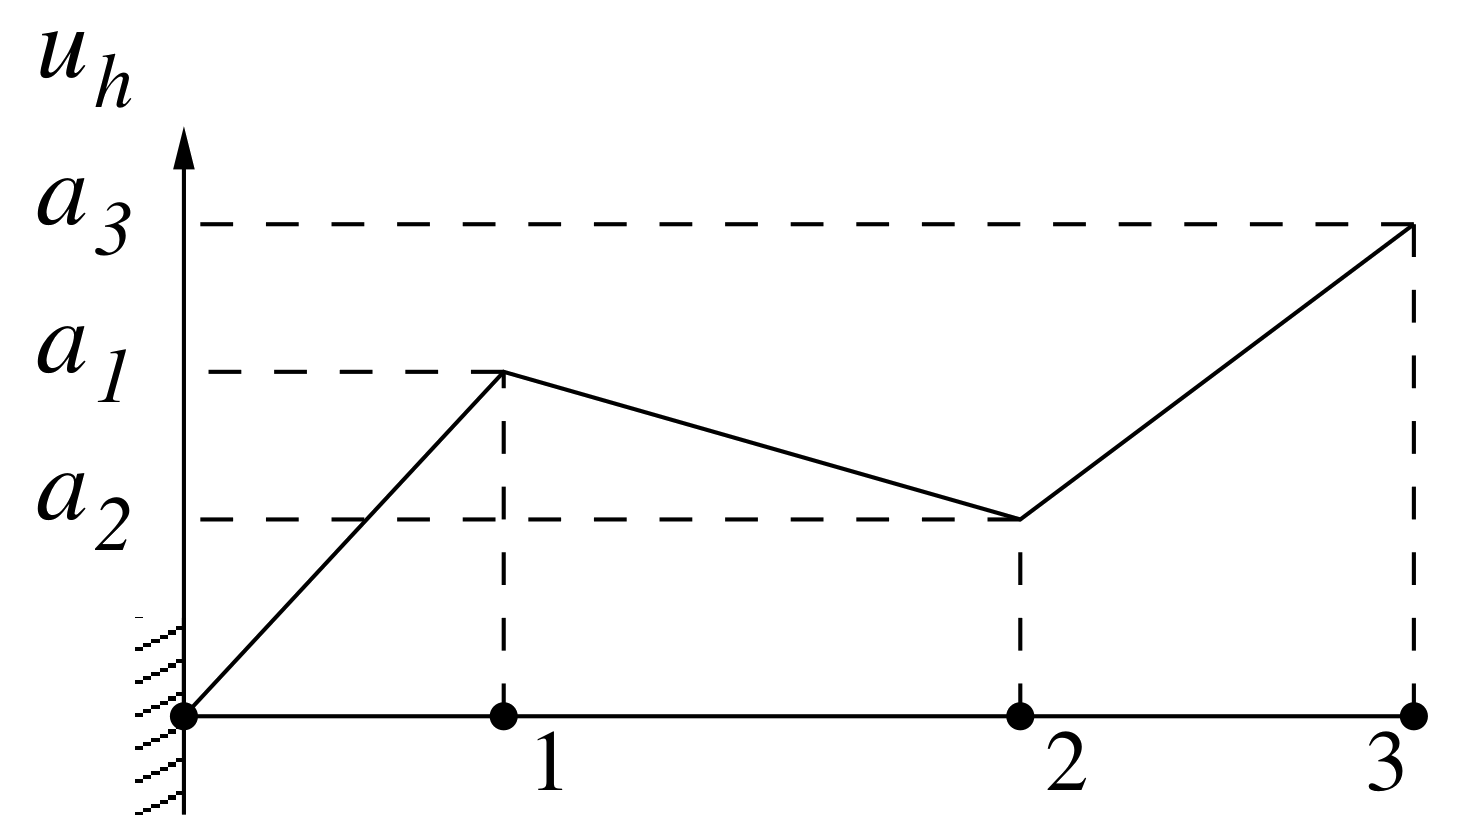
\includegraphics[width=\textwidth]{figs/beam-disp.png}
		\caption{displacement field}
	\end{subfigure}%
	\begin{subfigure}[b]{0.5\linewidth}
		\centering
		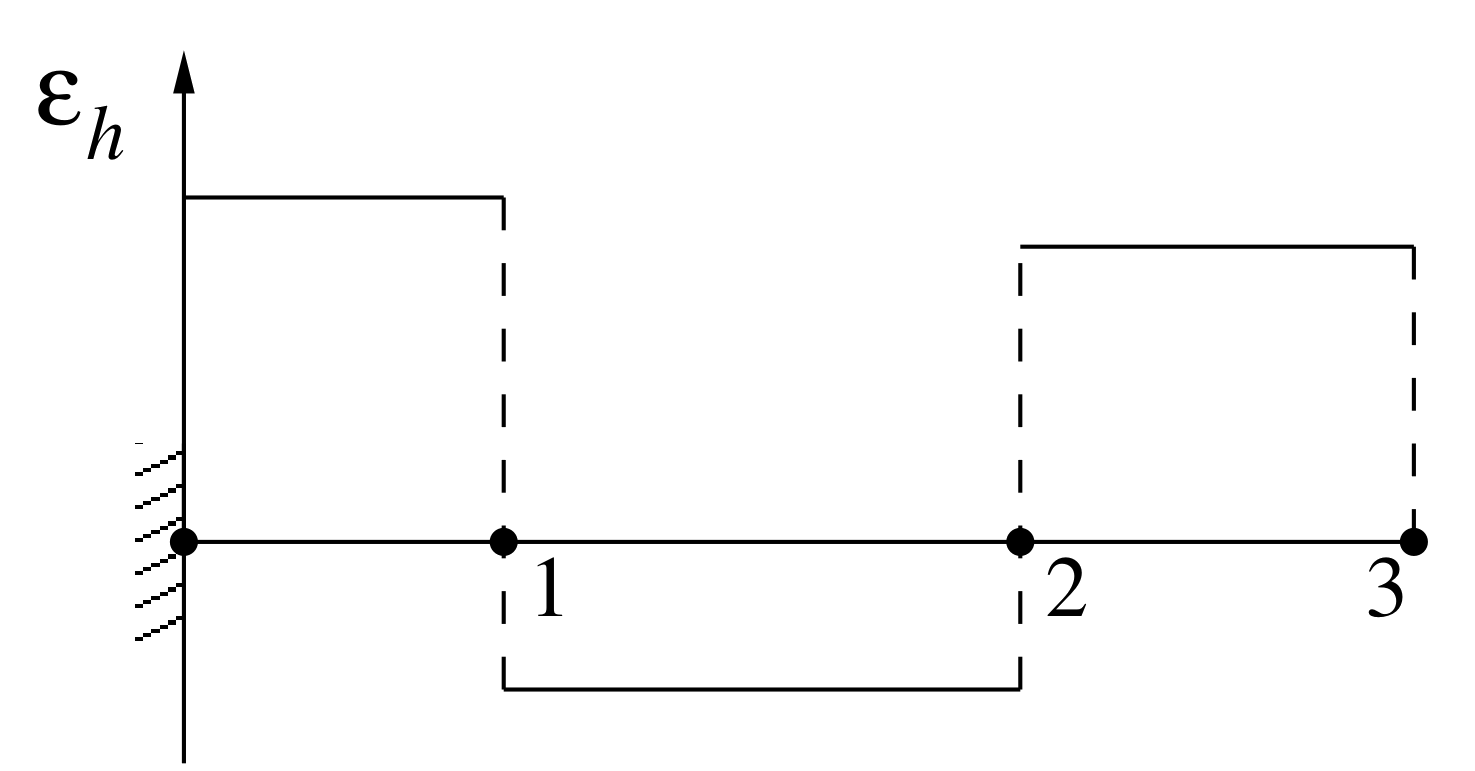
\includegraphics[width=\textwidth]{figs/beam-strains.png}
		\caption{strain field}
	\end{subfigure}
\end{figure}
\end{frame}

\note{
	An important point is the continuity of the approximate displacement field $u_h$. For the
	shape functions that we have introduced, the field $u_h$ is continuous, but its first derivative
	is discontinuous irrespective of the polynomial order of the basis functions. This is easy
	to see by considering two elements and computing the displacement and strain fields on
	either side of the node shared by the two elements.\\
	
	It does not matter how high the polynomial order of the shape functions is, the strain
	will be discontinuous at element boundaries.\\
	
	We can use these simple equations to construct shape functions that have discontinuous first
	derivatives in FEA of a bar because the weak form of the equation
	contains at most first-order derivatives. These shape functions are known as Lagrange
	polynomials. In the FEM, function with discontinuous derivatives are referred to as $C^0$ continuous functions. It turns out that these
	functions are not suitable for thin beam bending problems, and we will need to construct
	a different type of shape function for beams.
}

\note {
	For the two elements:
	the displacement at node 2 from the left-hand side is given by:
	\begin{equation*}
		u_h(x_2^-) = N_1(x_2)a_1 + N_2(x_2)a_2 = a_2
	\end{equation*}
	since $N_2 = 1$ at $x_2$ and all other shape functions are equal to zero. Similarly from the
	right-hand side of the node,
	\begin{equation*}
		u_h(x_2^+) = N_2(x_2)a_2 + N_3(x_2)a_3 = a_2
	\end{equation*}
	
	Now for the strain:
	\begin{equation*}
		\epsilon_h(x_2^-) = \frac{dN_1(x_2)}{dx}a_1 + \frac{dN_2(x_2)}{dx}a_2; \quad  \frac{dN_1(x_2)}{dx} \ne 0 \quad \mathrm{\&} \frac{dN_2(x_2)}{dx} \ne 0
	\end{equation*}
	\begin{equation*}
		\epsilon_h(x_2^+) = \frac{dN_2(x_2)}{dx}a_1 + \frac{dN_3(x_2)}{dx}a_2; \quad \frac{dN_2(x_2)}{dx} \ne 0 \quad \mathrm{\&} \frac{dN_3(x_2)}{dx} \ne 0
	\end{equation*}
	Clearly the strain is not continuous.
	

}
%------------------------------------------------
\begin{frame}
\frametitle{Quadratic element: shape functions}
\mode<beamer>{
\begin{figure}
	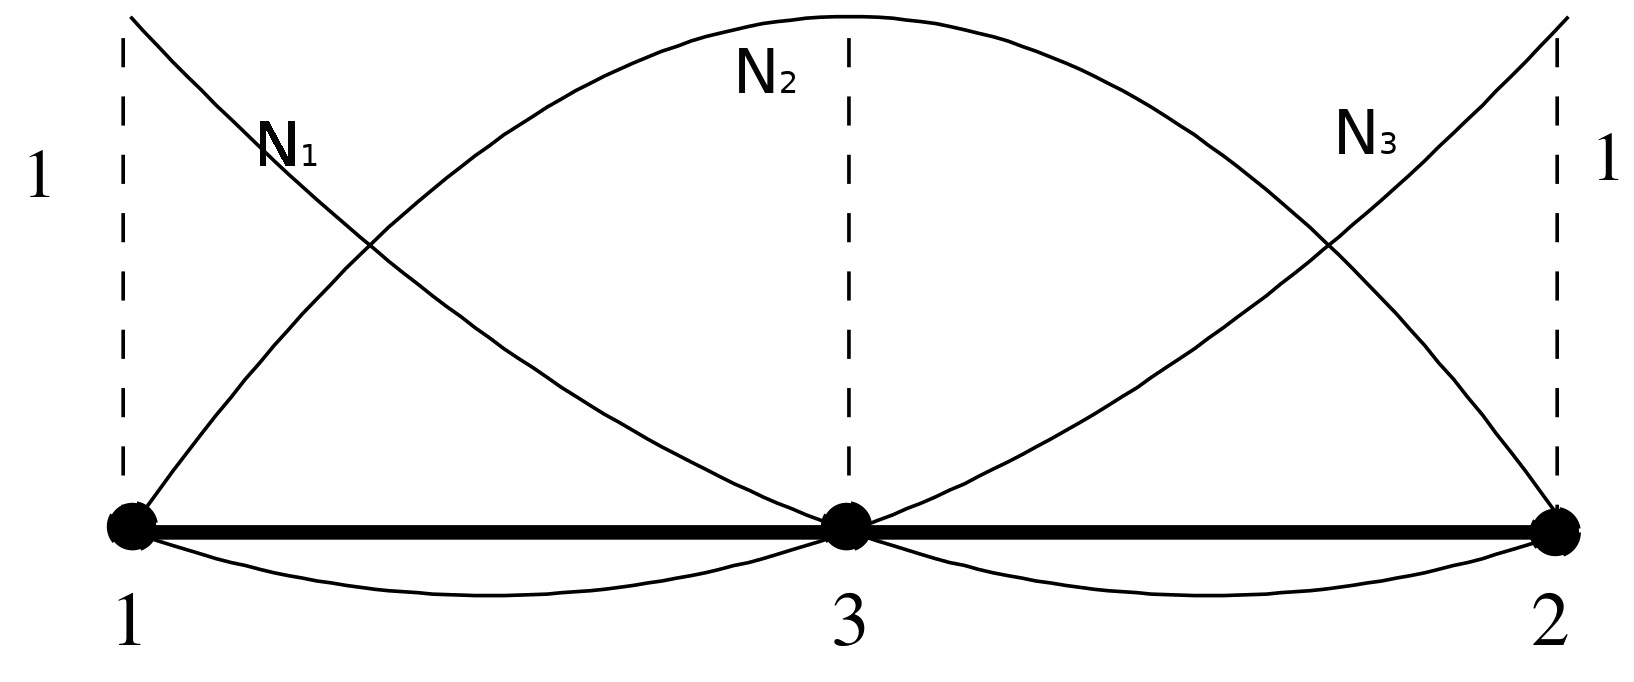
\includegraphics[width=0.5\textwidth]{figs/quadratic-shape-functions.png}
\end{figure}
}
\mode<handout>{
	\vspace{3cm}
}
\noindent
\fboxsep=0pt
\noindent
\begin{minipage}[t]{0.48\linewidth}
	The shape functions:
	\mode<beamer>{
		\begin{align*}
			N_1 & = a_1 + b_1 x + c_1 x^2 \,, \\
			N_2 & = a_2 + b_2 x + c_2 x^2 \,, \\
			N_3 & = a_3 + b_3 x + c_3 x^2
		\end{align*}
	}
	\mode<handout>{
		\vspace{1.5cm}
	}
\end{minipage}%
\hfill%
\begin{minipage}[t]{0.48\linewidth}
	$x_1 = -1$, $x_2 = 1$ and $x_3 = 0$:
	\mode<beamer>{
		\begin{align*}
			N_1 & = \frac{x^2}{2} - \frac{x}{2} \,, \\
			N_2 & = \frac{x^2}{2} + \frac{x}{2} \,, \\
			N_3 & = -x^2 + 1
		\end{align*}
	}
	\mode<handout>{
		\vspace{1.5cm}
	}
\end{minipage}
\end{frame}

%------------------------------------------------
\begin{frame}
\frametitle{Quadratic element: shape functions}
	The shape functions must satisfy three conditions and will be cubic polynomials of the form $N_i = a_i + b_i\, x + c_i\, x^2$. The SF must be equal to one at their node and zero at all others:
	\begin{equation*}
		\begin{bmatrix}
			1 & x_1 & x_1^2 \\
			1 & x_2 & x_2^2 \\
			1 & x_3 & x_3^2 \\
		\end{bmatrix}
		\begin{bmatrix}
			a_i \\
			b_i \\
			c_i \\
		\end{bmatrix}
		= %
		\begin{bmatrix}
			1 & -1 & 1 \\
			1 &  0 & 0\\
			1 &  1 & 1 \\
		\end{bmatrix}
		\begin{bmatrix}
			a \\
			b \\
			c \\
		\end{bmatrix}
		= 
		\begin{bmatrix}
			N_i(x_1) \\
			N_i(x_2) \\
			N_i(x_3) \\
		\end{bmatrix}
	\end{equation*}
Inverting,	
	\begin{equation*}
	\begin{bmatrix}
		 0   &  1 & 0   \\
        -0.5 &  0 & 0.5 \\
		 0.5 & -1 & 0.5 \\
	\end{bmatrix}
	\begin{bmatrix}
		N_i(x_1) \\
		N_i(x_2) \\
		N_i(x_3) \\
	\end{bmatrix} =
	\begin{bmatrix}
		a_i \\
		b_i \\
		c_i \\
	\end{bmatrix}
	\end{equation*}
For node one, $\left[N_i(x_1) \quad N_i(x_2) \quad N_i(x_3)\right]^T = \left[1 \quad 0 \quad 0 \right]^T$, and for node two $\left[0 \quad 0 \quad 1 \right]^T$, for node three $\left[0 \quad 1 \quad 0 \right]^T$. This leads to
	\begin{equation*}
		N_1 = \frac{x^2}{2} - \frac{x}{2} \,, \quad %
		N_2 = \frac{x^2}{2} + \frac{x}{2} \,, \quad %
		N_3 = -x^2 + 1
	\end{equation*}

\end{frame}
\end{document} 


